\documentclass[12pt,letterpaper,fleqn]{article}
\usepackage{fullpage}
\usepackage[top=2cm, bottom=4.5cm, left=2.5cm, right=2.5cm]{geometry}
\usepackage{amsmath,amsthm,amsfonts,amssymb,amscd}
\usepackage[utf8]{inputenc}
\usepackage{lastpage}
\usepackage{enumerate}
\usepackage{fancyhdr}
\usepackage{mathrsfs}
\usepackage{xcolor}
\usepackage{graphicx}
\usepackage{listings}
\usepackage{hyperref}
\usepackage{amsmath}
\usepackage{nccmath}
\usepackage{physics}
\usepackage{float}

\newcommand{\R}{\mathbb{R}}
\newcommand{\Q}{\mathbb{Q}}

\newcommand{\cent}{$^{\circ}$}
\newcommand{\delfrac}[2][y]{\frac{\partial #1}{\partial #2}}


\hypersetup{%
 colorlinks=true,
  linkcolor=blue,
  linkbordercolor={0 0 1}
}
 
\renewcommand\lstlistingname{Algorithm}
\renewcommand\lstlistlistingname{Algorithms}
\def\lstlistingautorefname{Alg.}

\lstdefinestyle{Python}{
    language        = Python,
    frame           = lines, 
    basicstyle      = \footnotesize,
    keywordstyle    = \color{blue},
    stringstyle     = \color{green},
    commentstyle    = \color{red}\ttfamily
}

\setlength{\parindent}{0.3in}
\setlength{\parskip}{0.05in}

% Edit these as appropriate
\newcommand\course{Física - Frente 1}
\newcommand\hwnumber{1}                  % <-- homework number
\newcommand\NetIDa{netid19823}           % <-- NetID of person #1
\newcommand\NetIDb{netid12038}           % <-- NetID of person #2 (Comment this line out for problem sets)

\pagestyle{fancyplain}
\headheight 35pt
%\lhead{\NetIDa}
%\lhead{\NetIDa\\\NetIDb}                 % <-- Comment this line out for problem sets (make sure you are person #1)
\chead{\textbf{\Large Tipos de Força \hwnumber}}
\rhead{\course \\ Maio/2020}
\lfoot{}
\cfoot{}
\rfoot{\small\thepage}
\headsep 1.5em

\begin{document}
\begin{itemize}
    \item \textbf{Força Elástica}
    
    \begin{enumerate}
        \item O dinamômetro, ou balança de mola, é um instrumento para medir força. Se graduado em newtons, ele indica o par de forças que é exercido sobre ele, distendendo a mola. Com a graduação em quilogramas é que ele se tornou conhecido no tempo do império como “balança de peixeiro”, pois o peixe era carregado em cestas sobre burros e comercializado pelas ruas. A figura a seguir mostra um dinamômetro de peso desprezível, em cujas extremidades estão aplicadas as forças indicadas.
        \begin{figure}[h]
            \centering
            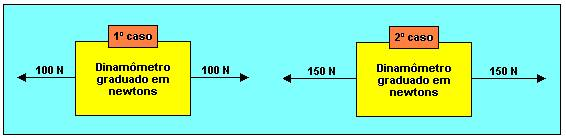
\includegraphics[width=0.8\textwidth]{ex_1.jpg}
        \end{figure}
        Assinale a alternativa correta.
        \begin{enumerate}
            \item A indicação do dinamômetro no primeiro caso é zero.
            \item A leitura do dinamômetro no segundo caso é 300 N.
            \item A resultante sobre o dinamômetro no primeiro caso é 100 N.
            \item A indicação do dinamômetro no primeiro caso é 100 N.
            \item A leitura do dinamômetro no segundo caso é 50 N.
        \end{enumerate}
        
        \item Durante os exercícios de força realizados por um corredor, é usada uma tira de borracha presa ao seu abdome. Nos arranques, o atleta obtém os seguintes resultados:
        \begin{table}[h]
            \centering
            \begin{tabular}{|c|c|c|c|c|c|}
            \hline
                 \textbf{Semana}&1&2&3&4&5  \\\hline
                 \textbf{$\Delta x$ (cm)}& 20&24&26&27&28  
                 \\ \hline
            \end{tabular}
        \end{table}
        
        O máximo de força atingido pelo atleta, sabendo-se que a constante elástica da tira é de 300 N/m e que obedece à lei de Hooke, é, em N,
        \begin{enumerate}
            \item 23520
            \item 17600
            \item 1760
            \item 840
            \item 84
        \end{enumerate}
        
        \item A mola da figura varia seu comprimento de 10cm para 22cm quando penduramos em sua extremidade um corpo de 4N.
        \begin{figure}[H]
            \centering
            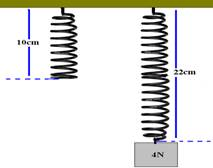
\includegraphics[width=0.3\textwidth]{ex_3.jpg}
        \end{figure}
        Determine o comprimento total dessa mola quando penduramos nela um corpo de 6N de peso.
        
        \item A mola da figura está:
        \begin{figure}[h]
            \centering
            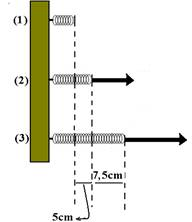
\includegraphics[width=0.3\textwidth]{ex_4.jpg}
        \end{figure}
        \begin{itemize}
            \item em (1) no seu tamanho natural
            \item em (2) tracionada por uma força de 10N
            \item em (3) tracionada por uma força de 25N
        \end{itemize}
        
        Verifique, justificando, se ela obedece à lei de Hooke.
        
        \textit{Dica: Lembre que a Lei de Hooke diz que a constante da mola é constante, ou seja, a força aumenta se a deformação for maior.}
        
        \item Sensores de dimensões muito pequenas têm sido acoplados a circuitos microeletrônicos. Um exemplo é um medidor de aceleração que consiste de uma massa m presa a uma micromola de constante elástica k. Quando o conjunto é submetido a uma aceleração a, a micromola se deforma, aplicando uma força F na massa (ver diagrama a seguir). O gráfico a seguir do diagrama mostra o módulo da força aplicada versus a deformação de uma micromola utilizada num medidor de aceleração.
        
        \begin{figure}[H]
            \centering
            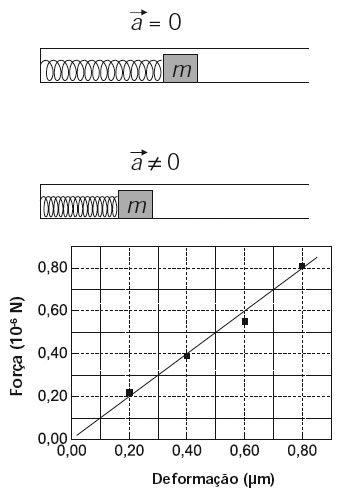
\includegraphics[width=0.3\textwidth]{ex_5.jpg}
        \end{figure}
        
        \begin{enumerate}
            \item Qual é a constante elástica k da micromola?
            \item O medidor de aceleração foi dimensionado de forma que essa micromola sofra uma deformação de 0,50 $\mu$m quando a massa tem uma aceleração de módulo igual a 25 vezes o da aceleração da gravidade. Qual é o valor da massa m ligada à micromola?
        \end{enumerate}
        
        \item Uma massa M=(20/9)kg, encontra-se suspensa ao conjunto de molas ilustrado na figura abaixo. Suas constantes elásticas são $k_1$ = $k_2$=30 N/m.
        
        \begin{figure}[h]
            \centering
            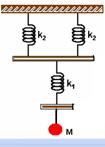
\includegraphics[width=0.25\textwidth]{ex_6.jpg}
        \end{figure}
        
        Calcule a constante elástica total equivalente do conjunto.
        
        \item Um corpo de massa m está suspenso por duas molas ideais, paralelas, com constantes elásticas k e deformadas de d.
        
        \begin{figure}[h]
            \centering
            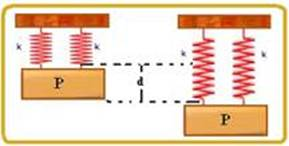
\includegraphics[width=0.3\textwidth]{ex_7.jpg}
        \end{figure}
Sabendo que o sistema se encontra em equilíbrio, assinale a alternativa que expressa k.

Dado: Considere a aceleração da gravidade g.
\begin{enumerate}
    \item $\frac{2mg}{d}$
    \item $\frac{mg}{d}$
    \item $\frac{mg}{2d}$
    \item $\frac{2d}{mg}$
    \item $mg$
\end{enumerate}
    \end{enumerate}
    
    \item \textbf{Força de tração}
    
    \begin{enumerate}
        \item Três blocos são atados por fios ideais e puxados no espaço interestelar, onde inexiste gravidade, com uma aceleração a de módulo $10m/s^2$.
        \begin{figure}[h]
            \centering
            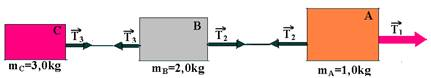
\includegraphics[width=0.6\textwidth]{ex_8.jpg}
        \end{figure}
        Quais as intensidades T1, T2 e T3 das forças tensoras nos fios?
        
        \textit{Dica: cada corpo acelera à $10\,m/s^2$. Fazer o diagrama de forças e usar a 2ª Lei de Newton para descobrir cada tração.}
        
        \item Dois corpos A e B de massas $m_A=3kg$ e $m_B=1kg$ estão ligados por um fio flexível, como mostra a figura,a mover-se sob a ação da gravidade, sem atrito. (considere $g=10m/s^2$).
        \begin{figure}[h]
            \centering
            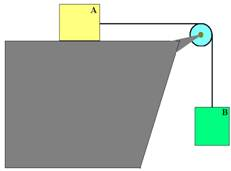
\includegraphics[width=0.4\textwidth]{ex_9.jpg}
        \end{figure}
        \begin{enumerate}
            \item Determine a aceleração do conjunto e a intensidade da força de tração no fio.
            \item Supondo que num certo instante, após iniciado o movimento, o fio de ligação se rompa, o que acontecerá com os movimentos dos corpos A e B
        \end{enumerate}
        
        \textit{Dica: Para o item (a), faça os esquemas de força em cada corpo e aplique a 2ª Lei de Newton.}
        
        \item Na montagem abaixo, sabendo-se que F=40N, $m_1=m_2=1,0kg$ e que $g=10\,m/s^2$, qual é o valor de T? Despreze qualquer atrito.
        \begin{figure}[h]
            \centering
            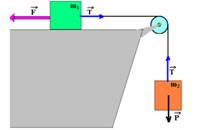
\includegraphics[width=0.5\textwidth]{ex_10.jpg}
        \end{figure}
        
        \item Dois carrinhos de supermercado podem ser acoplados um ao outro por meio de uma pequena corrente, de modo que uma única pessoa, ao invés de empurrar dois carrinhos separadamente, possa puxar o conjunto pelo interior do supermercado. Um cliente aplica uma força horizontal de intensidade F, sobre o carrinho da frente, dando ao conjunto uma aceleração de intensidade $0,5 m/s^2$.
        \begin{figure}[h]
            \centering
            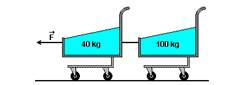
\includegraphics[width=0.4\textwidth]{ex_11.jpg}
        \end{figure}
        
        Sendo o piso plano e as forças de atrito desprezíveis, o módulo da força F e o da força de tração na corrente são, em N, respectivamente:
        \begin{enumerate}
            \item 70 e 20
            \item 70 e 40
            \item 70 e 50
            \item 60 e 20
            \item 60 e 50
        \end{enumerate}
        
        \item Dois blocos, A e B, de massas m e 2m, respectivamente, ligados por um fio inextensível e de massa desprezível, estão inicialmente em repouso sobre um plano horizontal sem atrito. Quando o conjunto é puxado para a direita pela força horizontal  aplicada em B, como mostra a figura, o fio fica sujeito à tração $T_1$. Quando puxado para a esquerda por uma força de mesma intensidade que a anterior, mas agindo em sentido contrário, o fio fica sujeito à tração $T_2$.
        \begin{figure}[h]
            \centering
            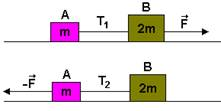
\includegraphics[width=0.5\textwidth]{ex_12.jpg}
        \end{figure}
        
        Nessas condições, pode-se afirmar que $T_2$‚ é igual a:
        \begin{enumerate}
            \item $2\,T_1$ 
            \item $\sqrt{2}\,T_1$
            \item $T_1$
            \item $\frac{T_1}{\sqrt{2}}$
            \item $\frac{T_1}{2}$
        \end{enumerate}
        
        \item Analise as figuras a seguir e leia com atenção o texto.
        \begin{figure}[h]
            \centering
            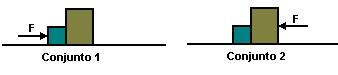
\includegraphics[width=0.6\textwidth]{ex_13.jpg}
        \end{figure}
        
        Dois blocos de massas m e M, sendo $M>m$ estão em repouso e em contato um ao lado do outro, sobre uma superfície plana. Se empurrarmos um dos blocos com uma força F, paralela à superfície, o conjunto irá mover-se com uma dada aceleração.
        
Determine se faria diferença para as magnitudes da aceleração do conjunto e das forças de contato entre os blocos, se tivéssemos empurrado o outro bloco.
    \end{enumerate}
    
    \item \textbf{Força de Atrito}
    
    \textbf{Atenção:} Há 2 tipos de coeficientes de atritos:
    \begin{itemize}
        \item $\mu_e$ - coeficiente de atrito estático: é quando o objeto não está em movimento. Nesse caso, a força de atrito é igual a força aplicada para tentar colocar o objeto em movimento. Existe uma força de atrito estático limite, que é quando qualquer força maior que esta é aplicada, o objeto entra em movimento e atrito vira dinâmico.
        
        Ela é dada por: $(F_{at})_{lim} = \mu_e*N$ - em que N é a força normal;
    \item$\mu_d$ - coeficiente de atrito dinâmico: é quando o objeto está em movimento. Nesse caso a força de atrito é dada por: $F_{at} = \mu_d*N$, em que N é a normal 
    \end{itemize}
    
    \begin{enumerate}
        \item Um bloco de borracha de massa 5,0 kg está em repouso sobre uma superfície plana e horizontal. O gráfico representa como varia a força de atrito sobre o bloco quando sobre ele atua uma força F de intensidade variável paralela à superfície.
        
        \begin{figure}[h]
            \centering
            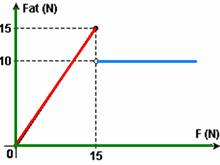
\includegraphics[width=0.4\textwidth]{ex_14.jpg}
        \end{figure}
        
        O coeficiente de atrito estático entre a borracha e a superfície, e a aceleração adquirida pelo bloco quando a intensidade da força atinge 30N são, respectivamente, iguais a:
        \begin{enumerate}
            \item $0,3\quad e \quad 4,0\, m/s^2$
            \item $0,2\quad e \quad 6,0\, m/s^2$
            \item $0,3\quad e \quad6,0\, m/s^2$
            \item $0,5\quad e \quad 4,0\, m/s^2$
            \item $0,2\quad e \quad3,0\, m/s^2$
        \end{enumerate}
        
        \item Uma caixa cuja velocidade inicial é de 10 m/s leva 5 s deslizando sobre uma superfície horizontal até parar completamente.

Considerando a aceleração da gravidade $g = 10 m/s^2$, determine o coeficiente de atrito cinético que atua entre a superfície e a caixa.

\begin{enumerate}
    \item 0,1 
    \item 0,2
    \item 0,3
    \item 0,4
    \item 0,5
\end{enumerate}

\item Dois carros de corrida são projetados de forma a aumentar o atrito entre os pneus e a pista. Os projetos são idênticos, exceto que num deles os pneus são mais largos e no outro há um aerofólio. Nessas condições podemos dizer que:

\begin{enumerate}
    \item nenhum dos projetos alterará o atrito.
    \item o atrito será maior no carro com aerofólio.
    \item em ambos os projetos, o atrito será aumentado em relação ao projeto original.
    \item em ambos os projetos, o atrito será diminuído em relação ao projeto original.
    \item o atrito será maior no carro com pneus mais largos.
\end{enumerate}

\item Um caixote de massa 20kg está em repouso sobre a carroceria de um caminhão que percorre uma estrada plana, horizontal, com velocidade constante de 72km/h. Os coeficientes de atrito estático e dinâmico entre o caixote e o piso da carroceria, são aproximadamente iguais e valem $\mu=0,25$ (admitir $g=10m/s^2$)

\begin{enumerate}
    \item Qual é a intensidade da força de atrito que está agindo sobre o caixote? Justifique.
    \item Determine o menor tempo possível para que esse caminhão possa frear sem que o caixote escorregue.
\end{enumerate}

\item Um automóvel de massa $10^3$ kg, movendo-se inicialmente com velocidade de 72km/h é freado (em movimento uniformemente desacelerado) e pára, após percorrer 50m. Calcule a força, o tempo de freamento e o valor do coeficiente de atrito. ($g=10m/s^2$)

    \end{enumerate}
\end{itemize}
\newpage
\section*{GABARITO}
\begin{itemize}
    \item \textbf{Força Elástica}
\begin{enumerate}
    \item (d) - a Resultante é zero, mas a indicação do dinamômetro é o quanto de força que ele aplica no objeto, que é 100 N
    
    \item (e)
    \item Vamos analisar o primeiro corpo. Como a mola vai compensar a força peso, então $F_{el} = -4N$ (onde o sinal de menos é porque a direção da força elástica é oposta a da força peso). Pela Lei de Hooke, então:
    \begin{align*}
        F_{el} = -k*\Delta x \\
        -4 = -k*(22-10)\\
        k = 4/12 = \frac{1}{3}\, N/cm
    \end{align*}
    Com isso, podemos achar o quanto a mola deforma para o corpo de 6N. Como a força elástica está em oposição à força peso: $F_{el}= -6 N$. Então, pela Lei de Hooke:
    \begin{align*}
        F_{el}=-k\Delta x \\
        -6 = -\frac{1}{3} \Delta x \\
        \Delta x = 18 cm
    \end{align*}
    Como o $\Delta x$ é: $\Delta x = x - x_i$, em que 'x' é o comprimento final e $x_i$ é o comprimento relaxado da mola.
    Logo:
    \begin{align*}
        18 = x - 10 \implies \boxed{x = 28 cm}
    \end{align*}
    
    \item Pela Lei de Hooke, a constante da mola é uma constante, ou seja, a força é proporcional à deformação. Por isso, podemos falar que:
    \begin{align*}
        F_{el} = -k\Delta x \implies k = -\frac{F_{el}}{\Delta x}
    \end{align*}
    
    Como o problema é feito sobre uma mesma mola, para a mola respeitar a Lei de Hooke, o 'k' dela tem que ser o mesmo para os dois casos, ou seja:
    \begin{align*}
        -\frac{F_{el1}}{\Delta x_1} = -\frac{F_{el2}}{\Delta x_2}
    \end{align*}
    No primeiro caso, o exercício diz que a força é de 10 N e pela imagem, a deformação é de 5cm. No segundo caso, a força é dita ser de 25N e a deformação, pela imagem, é de 12,5 cm, portanto:
    \begin{align*}
        \frac{10}{5} = \frac{25}{12,5} \implies 2 =2
    \end{align*}
    
    Portanto, sim, a mola respeita a Lei de Hooke.
    
    \item
    \begin{enumerate}
        \item Lembremos que o gráfico está na escala $10^{-6}$ N e que $\mu m$ é $10^{-6}$ m. Pegando a origem, (0,0), e o ponto (0.2, 0.2) para calcular a constante da mola:
        \begin{align*}
            k = \frac{(0,2 - 0)10^{-6}}{(0,2-0)10^{-6}} = 1 N/m
        \end{align*}
        
        \item Lembremos que a Lei de Hooke é uma força, logo subtituímos o módulo dela na 2ª Lei de Newton (porque temos somente a magnitude da força e da aceleração no enunciado):
        \begin{align*}
            |-k \Delta x| = m*a
        \end{align*}
        Colocando os dados da questão: $a = 25*g = 250 m/s^2$; $k=1 N/m$ e $\Delta x = 0,5  \mu m = 0,5*10^{-6}m$:
        \begin{align*}
            &1*0,5 *10^{-6} = m*250 \\
            &m = \frac{5*10^{-7}}{2,5*10^2} \implies m = 2*10^{-9} kg \implies m = 2*10^{-6} g  \implies m = 2\, \mu g
        \end{align*}
    \end{enumerate}
    \item As molas $k_2$ estão em paralelo, logo, a constante de mola equivalente delas é: $k_{eq2} = 30 + 30 = 60 N/M$. Agora o sistema será:
    \begin{figure}[h]
        \centering
        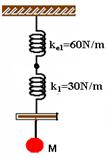
\includegraphics[width=0.2\textwidth]{resolucao_6.jpg}
    \end{figure}
    
    O nosso novo sistema é são 2 molas em série, logo a constante de mola equivalente será de:
    \begin{align*}
        &\frac{1}{k_{eq}} = \frac{1}{k_{eq2}} + \frac{1}{k_{1}} \\ &\frac{1}{k_{eq}} = \frac{1}{60} + \frac{1}{30}\\
        &\frac{1}{k_{eq}} = \frac{1 + 2}{60} = \frac{3}{60}\\
        &\implies k_{eq} = \frac{60}{3} = 20 N/m
    \end{align*}
    
    \item Como o sistema está em equilíbrio, a força peso deve ser igual à força elástica. Como são duas molas em paralelo, então a constante de mola equivalente é: $k_{eq} = k+k = 2k$ Portanto:
    \begin{align*}
        &F_el + P =0 \\
        &-2kd + mg =0 \\
        & 2kd =mg \implies k = \frac{mg}{2d}
    \end{align*}
    Logo, letra (c)
\end{enumerate}

\item \textbf{Força de Tração}

\begin{enumerate}
    \item Comecemos pelo primeiro corpo. Nele só tem a força de tração $T_3$ aplicada, então pela 2ª Lei de Newton:
    \begin{align*}
        &F = m_c*a \\
        &T_3 = 3*10 = 30 N
    \end{align*}
    
    Olhemos, agora, para o segundo corpo:
    \begin{align*}
        &T_2 - T_3 = 2*10 \\
        & T_2 = 20 + 30 = 50 N
    \end{align*}
    
    Por fim, o último corpo:
    \begin{align*}
        &T_1 - T_2 = 1*10 \\
        &T_1 = 10+ 50 = 60 N
    \end{align*}
    Enfim:
    \begin{equation*}
        \boxed{\begin{split}
            &T_1 = 30\, N\\
            &T_2 = 50\, N\\
            &T_3 = 60\, N
        \end{split}}
    \end{equation*}
    
    \item \begin{enumerate}
    O esquema de forças é:
    \begin{figure}[h]
        \centering
        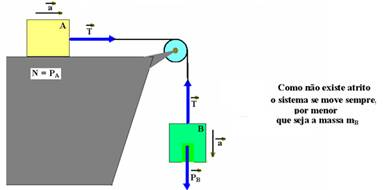
\includegraphics[width=0.6\textwidth]{resolucao_9.jpg}
    \end{figure}
    
        \item O conjunto vai ter a mesma aceleração, pois os blocos estão conectados por um cabo. Para o corpo A, só há a força de tração puxando, então:
        \begin{align*}
            T = 3*a
        \end{align*}
        
        Para o corpo B, as forças agindo nele são a força peso, puxando para baixo e a tração puxando para cima, então:
        \begin{align*}
            &P - T = 1*a \\
            &1*10 - T = a
        \end{align*}
        
        Substituindo o T, pela fórmula achada no corpo A:
        \begin{align*}
            10 - 3a = a \implies 4a = 10 \implies a =2,5\,m/s^2
        \end{align*}
        
        Substituindo 'a' de volta, vemos que a tração será:
        \begin{align*}
            T =3*2,5 \implies T = 7,5 N
        \end{align*}
        
        \item Quando se rompe o cabo, o bloco A não terá força aplicada nele, logo a aceleração dele será 0, assim o bloco fica no Movimento Retilíneo Uniforme até colidir com a polia. Já o bloco B, só restará a força peso, que fará o bloco cair em queda livre com a aceleração igual à $g=10\,m/s^2$.
    \end{enumerate}
    
    \item Por causa que os corpos estão conectados por uma cabo, a aceleração deles deve ser a mesma. No corpo 1, a 2ª Lei de Newton é:
    \begin{align*}
        &T - F =1*a\\
        &T = a +40
    \end{align*}
    
    No corpo 2, a 2ª Lei de Newton será:
    \begin{align*}
        &P - T = 1*a\\
        &1*10 = a + T = a + a+ 40 \\
        &2a=10 - 40 = -30\implies a = -15m/s^2
    \end{align*}
    
    Subtituindo 'a' na primeira fórmula, temos que:
    \begin{align*}
        T = -15 + 40 \implies \boxed{T = 25 N}
    \end{align*}
    
    \item Lembre que como o corpo está conectado pelo cabo, então os dois tem a mesma aceleração, de $0,5\,m/s^2$
    
    No corpo da direita, a 2ª Lei de Newton é:
    \begin{align*}
        &F_{res} = m*a\\
        &T = 100*0,5 = 50 N
    \end{align*}
    
    No corpo da esquerda:
    \begin{align*}
        &F_{res} = m*a\\
        & F - T = 40*0,5\\
        &F = 20 + 50 = 70 N
    \end{align*}
    Logo, letra (c)
    
    \item Lembrar que como os corpos estão conectados, a aceleração deles é igual (a). Analisando o primeiro caso para o corpo A:
    \begin{align*}
        &F_{res} = m_A*a \\
        &T_1 = ma
    \end{align*}
    Olhando para o corpo B, no segundo caso:
    \begin{align*}
        &F_{res} = 2m(-a)\\
        &-T_2 = 2m(-a)\\
        &T_2= 2ma
    \end{align*}

    Comparando as trações, vemos que $T_2 = 2T_1$, logo (a).
    
    \item Para a aceleração do objeto, como a única força externa aplicada é a F nos dois casos e a massa total é $m+M$, então a aceleração do conjunto tem que ser a mesma em ambos os casos, pela 2ª Lei de Newton.
    
    Mas as forças de contato serão diferentes. No primeiro caso, o objeto de massa M é que tá sendo empurrado para frente pela força de contato, e como a aceleração é única, então a 2ª Lei de Newton fica:
    \begin{align*}
        N_1 = M*a
    \end{align*}
    
    No segundo caso, o bloco de massa 'm' é que tá sendo empurrado pela força de contato e, como a aceleração é única, então:
    \begin{align*}
        N_2 = m*a
    \end{align*}
    Como a aceleração é única e $M>m$, então $N_1>N_2$, o que nos mostra que a força de contato nos casos são diferentes.
\end{enumerate}

\item \textbf{Força de Atrito}

\begin{enumerate}
    \item Pelo gráfico, percebemos que o atrito limite é quando $F_{at} = 15$ N, então pela fórmula do atrito limite:
    \begin{align*}
        15=\mu_e*N
    \end{align*}
    Como a superfície é plana e horizontal, então $N = P = mg$, logo:
    \begin{align*}
        N = 5*10 = 50 N
    \end{align*}
    Então
    \begin{align*}
        15 = \mu_e*50 \implies \boxed{\mu_e = 0,3}
    \end{align*}
    
    Para uma força de 30 N, o atrito se torna dinâmico e a força de atrito é de 10 N. Logo:
    \begin{align*}
        &F - F_{at} = m*a \\
        &30 - 10 = 5*a \\
        &a = \frac{20}{5} \implies \boxed{a= 4\,m/s^2}
    \end{align*}
    
    Logo, letra (a)
    
    \item Usando a equação da velocidade para determinar a aceleração da frenagem da caixa:
    
    \begin{align*}
        &V=V_0 + at \\
        &0=10 + a*5 \implies a =-2\,m/s^2
    \end{align*}
    
    Com isso, pela 2ª Lei de Newton, a força da frenagem será de:
    \begin{align*}
        &F=ma\\
        &F =-2*m
    \end{align*}
    
    Como a caixa deslizou na superfície, então o atrito é dinâmico/cinético, então a força de atrito é dada por:
    \begin{align*}
        F_{at} = \mu_c*N
    \end{align*}
    Como a caixa está numa superfície horizontal, a normal é igual ao peso: $N=m*g=10m$. Substituindo os valores:
    \begin{align*}
        2m= \mu_c*10m \\
        &2=10\mu_c \implies \boxed{\mu_c = 0,2}
    \end{align*}
    Logo, letra (b)
    \item (c)
    
    \item \begin{enumerate}
        \item A força de atrito será 0, porque o caminhão está andando a uma velocidade constante, logo a aceleração é 0 e, assim, a força resultante é 0.
        
        \item Para que caixa não deslize enquanto o caminhão freia, a força de atrito tem que ser igual a força de frenagem do caminhão. Para que o caminhão pare o mais rápido possível sem a caixa deslizar, o atrito estático da caixa tem que ser o máximo, ou seja, o limite. Então:
        \begin{align*}
            (F_{at})_{lim} = \mu*N \\
        \end{align*}
        Como a superfície é horizontal: $N = P = mg$, então:
        \begin{align*}
            F_{at} = 0,25*20*10 = 50 N
        \end{align*}
        
        Então, a força de frenagem do caminhão tem que 50 N. Usando a 2ª Lei de Newton para descobrir a desaceleração da caixa/caminhão:
        \begin{align*}
            &F = m*a\\
            &-50 = 20*a \implies a = -2,5 \, m/s^2
        \end{align*}
        
        Logo, usando a equação da velocidade para saber quanto tempo demora a frenagem até parar completamente:
        \begin{align*}
            &V = V_0 + at\\
            &0 = V_0 -2,5*t
        \end{align*}
        Como a velocidade inicial do caminhão é 72 km/h $\rightarrow$ 20 m/s:
        \begin{align*}
            &0=20-2,5t \\
            &t = \frac{20}{2,5} \implies\boxed{t = 8s}
        \end{align*}
    \end{enumerate}
    \item Primeiramente, vamos achar a desaceleração do veículo. Para isso, vamos usar a Equação de Torricelli:
    \begin{align*}
        &v^2 = v_0^2 + 2a\Delta S\\
    \end{align*}
    
    Lembrando que 72km/h $\rightarrow$ 20m/s e, como ele para após $\Delta S=50$ m, então v=0:
    \begin{align*}
        &0 = 20^2 + 2*a*50 \\
        &100a = -400 \implies a =-4m/s^2
    \end{align*}
    Com isso, usando a equação da velocidade para achar o tempo de frenagem:
    \begin{align*}
        &v=v_0+at\\
        &0=20-4*t \implies \boxed{t = 5s}
    \end{align*}
    Colocando a aceleração na 2ª Lei de Newton:
    \begin{align*}
        &F=ma\\
        &F=1000*(-4) \implies \boxed{F=-4000 N}
    \end{align*}
    
    Como a frenagem é feita pela força de atrito:
    \begin{align*}
        F_{at}=\mu*N
    \end{align*}
    Supondo que o automóvel esteja num superfície horizontal, $N=P=mg=1000*10=10000\,N$:
    \begin{align*}
        4000 = \mu*10000 \implies \boxed{\mu =0,4}
    \end{align*}
\end{enumerate}
\end{itemize}
\end{document}
